
\begin{definition}[Diagram \cite{barr1990category}]
    \label{def:cat:diagram}
    Let \( G \) be an unlabeled graph. A \textbf{diagram} (in \( \mathcal{C} \) of shape \( G \)) is a homomorphism of unlabeled graphs \( h : G \mathop{\to} C \) where \( C \) is the underlying unlabeled graph of the category \( \mathcal{C} \). A diagram is \textbf{commutative} if, for all nodes \( u \), \( v \), and any two paths from \( u \) to \( v \) in the unlabeled graph \( G \):

    \begin{center}
    \resizebox{12cm}{!}{
        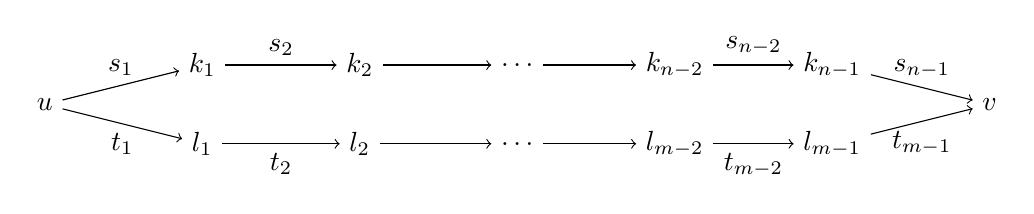
\begin{tikzpicture}
        \node (u) at (0,0) {\( u \)};
        \node (k1) at (2,0.5) {\( k_1 \)};
        \node (k2) at (4,0.5) {\( k_2 \)};
        \node (ketc) at (6,0.5) {\( \dots \)};
        \node (knm2) at (8,0.5) {\( k_{n-2} \)};
        \node (knm1) at (10,0.5) {\( k_{n-1} \)};
        \node (v) at (12,0) {\( v \)};
        \node (l1) at (2,-0.5) {\( l_1 \)};
        \node (l2) at (4,-0.5) {\( l_2 \)};
        \node (letc) at (6,-0.5) {\( \dots \)};
        \node (lnm2) at (8,-0.5) {\( l_{m-2} \)};
        \node (lnm1) at (10,-0.5) {\( l_{m-1} \)};
        \draw[->] (u) -- (k1) node [midway,above] {\( s_1 \)};
        \draw[->] (k1) -- (k2) node [midway,above] {\( s_2 \)};
        \draw[->] (k2) -- (ketc);
        \draw[->] (ketc) -- (knm2); 
        \draw[->] (knm2) -- (knm1) node[midway,above] {\( s_{n-2} \)}; 
        \draw[->] (knm1) -- (v) node[midway,above] {\( s_{n-1} \)}; 
        \draw[->] (u) -- (l1) node[midway,below] {\( t_1 \)};
        \draw[->] (l1) -- (l2) node[midway,below] {\( t_2 \)};
        \draw[->] (l2) -- (letc);
        \draw[->] (letc) -- (lnm2); 
        \draw[->] (lnm2) -- (lnm1) node[midway,below] {\( t_{m-2} \)}; 
        \draw[->] (lnm1) -- (v) node[midway,below] {\( t_{m-1} \)}; 
        \end{tikzpicture}
    }
    \end{center}
    \noindent
    the equality \( h(s_1) \mathop{\star} h(s_2) \mathop{\star} \dots  \mathop{\star} h(s_{n-1}) \mathop{=} h(t_1) \mathop{\star} h(t_2) \mathop{\star} \dots  \mathop{\star} h(t_{m-1}) \) holds.
\end{definition}